% figures-es/five-forces.tex
% Standalone TikZ: diagrama de las Cinco Fuerzas de Porter (ch.11 análisis competitivo).
% Compilado a figures-es/five-forces.pdf via tools/build-figures-es.sh.
\documentclass[tikz,border=4pt]{standalone}
\usepackage{tikz}
\usetikzlibrary{arrows.meta,positioning,calc}

\definecolor{vcblue}{HTML}{1A5276}
\definecolor{vcteal}{HTML}{0E6655}
\definecolor{vcgray}{HTML}{4D4D4D}

\begin{document}
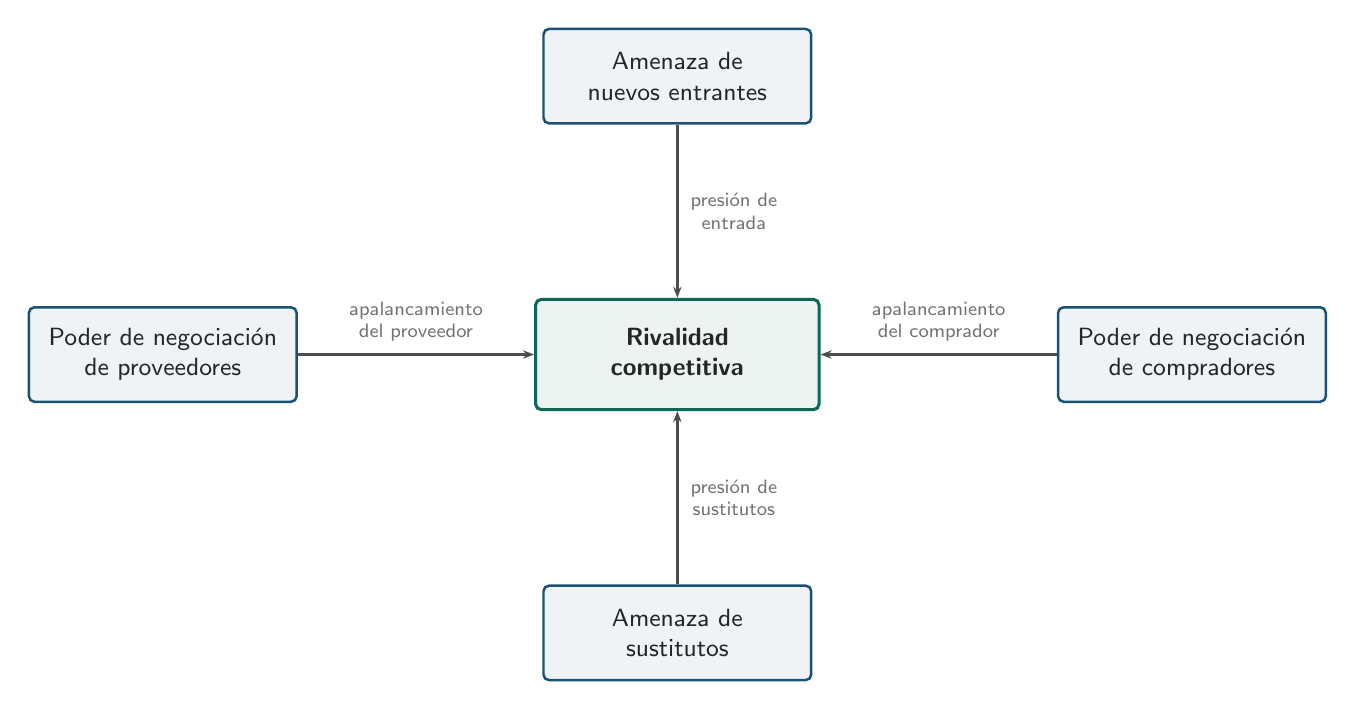
\begin{tikzpicture}[
  node distance=18mm,
  force/.style={draw=vcblue, line width=0.9pt, rounded corners=2pt, fill=vcblue!7,
                font=\sffamily\small, align=center,
                minimum width=34mm, minimum height=12mm, text=black!85},
  rivalry/.style={draw=vcteal, line width=1.1pt, rounded corners=2pt, fill=vcteal!8,
                  font=\sffamily\small\bfseries, align=center,
                  minimum width=36mm, minimum height=14mm, text=black!85},
  arr/.style={-{Stealth[length=4pt]}, vcgray, line width=0.9pt},
  lbl/.style={font=\sffamily\scriptsize, text=black!55, align=center},
]

%% Centro: rivalidad
\node[rivalry] (rival) {Rivalidad\\competitiva};

%% Cuatro fuerzas circundantes
\node[force, above=22mm of rival] (entry)   {Amenaza de\\nuevos entrantes};
\node[force, below=22mm of rival] (sub)     {Amenaza de\\sustitutos};
\node[force, left=30mm of rival]  (supplier){Poder de negociación\\de proveedores};
\node[force, right=30mm of rival] (buyer)   {Poder de negociación\\de compradores};

%% Flechas apuntando hacia el centro (rivalidad)
\draw[arr] (entry.south)   -- node[lbl, right=1pt] {presión de\\entrada} (rival.north);
\draw[arr] (sub.north)     -- node[lbl, right=1pt] {presión de\\sustitutos} (rival.south);
\draw[arr] (supplier.east) -- node[lbl, above=1pt] {apalancamiento\\del proveedor} (rival.west);
\draw[arr] (buyer.west)    -- node[lbl, above=1pt] {apalancamiento\\del comprador} (rival.east);

\end{tikzpicture}
\end{document}
